\chapter{Hardware Design}
\label{ch:hw_design}
We decided to design and implement two unique RocketCore CPUs for the heterogeneous SoC. These will be in two separate tiles with cache coherency. The aim will be for each core to implement the RV64GC ISA, the 'general-purpose' RISC-V ISA, as well as an MMU (Memory Management Unit) in order to run a full Debian Linux OS, if only with terminal interaction. The following code snippets show the parameterisation options available for the RocketCore CPU and the tiles they lie within.

%todo include core params and tile params code listing here

The micro-architecture specification of RocketCore is not publicised. This means implementation details of the core are not documented, and makes understanding how the core functions a difficult task. For example, to identify what changes occur when \texttt{useVM} is enabled instead of disabled, we must search through the source code (10000+ lines of Chisel\cite{}) to find where the value is used and what it is used for - what other variables are impacted, how they change, etc. The following sections identify and discuss what customisation is available, with parameters common between all cores specified and parameters that will be varied during testing identified.
%todo cite above
\section{Constant elements in RocketCore}
\subsection{Core Frequency - \texttt{bootFreqHz}}
The \texttt{bootFreqHz} core variable does not impact the actual frequency of the core, but instead is added to the device tree structure, so that an operating system is able to read the boot frequency of the CPU. The actual frequency of the cores are defined by clocks generated in the Vivado project. These can be edited, with supported frequencies of 160, 125, 100, 80, 62.5, 50, 40, 31.25, 25, and 20 MHz. The clock manager uses phase locked loop and counters to divide the central clock from the FPGA crystal oscillator. This reduces the available frequencies to those that can be formed from that central clock using the dividers. The Nexys-A7-100t has a crystal capable of generating up to 50 MHz, and is shared between all cores in the RocketChip SoC. This prevents individual clock frequencies for cores, one of the significant changes between big and small cores in typical heterogeneous systems. This will severely limit the actual performance difference between cores, as well as the power consumption difference. This also prevents frequency scaling as the RocketChip SoC does not have control of the clock generator, another key part of modern power saving measures. These are limitations of FPGAs as a platform and the SoC generators used in this project.

\begin{figure}
    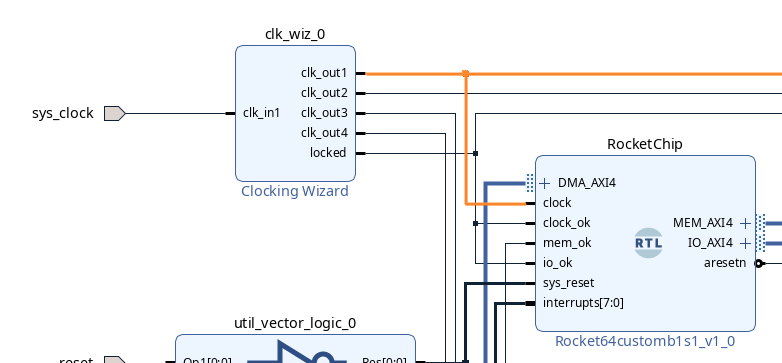
\includegraphics[width=0.8\textwidth]{./img/single_clock_rocketchip.png}
\end{figure}

\subsection{ALU}
The integer ALU is not customisable within RocketCore. This results in all RocketCore CPUs having the same integer additions per cycle, and as we cannot vary the frequency between cores in the FPGA, all our designs will have the same integer operations per second.

\subsection{}

\section{MMU}
The \texttt{useVM} option for core parameters controls whether an MMU (Memory Management Unit) is instantiated inside the core and virtual memory is used. MMU is enables the use of Virtual Memory, an abstraction of physical addresses to logical addresses. This increases the security and stability of a system, by preventing processes from accessing the memory space of other processes. Stopping reads to another processes' memory space ensures sensitive data currently held in memory by a process cannot be accessed by another process. Stopping writes to the memory space prevents the corruption of another processes' data, that could otherwise lead to user data loss, the process stopping unexpectedly or entire system crash depending on the importance of the memory corrupted process. Virtual memory can also allow more logical memory than there is physical memory to be allocated to programs.

The MMU in RocketCore is non-parameterisable - it is either instantiated inside the CPU or it isn't. We have chosen to enable virtual memory and have an MMU instantiated inside the cores. Support for the Linux kernel and Debian requires an MMU, hence it is needed in the cores. %todo include LUT comparison with enabled/disabled

\section{User/Supervisor modes}
The \texttt{useUser} and \texttt{useSupervisor} options control the addition of hardware privilege levels. All RISC-V CPUs have the machine privilege level (M-mode). Code run in M-mode is able to execute any instruction, including those that would result in the CPU becoming trapped permanently. M-mode is intended to be used for managing secure execution done in lower privilege levels, completely trusted code that must be run on M-mode for system setup or for embedded systems where M-mode is the only privilege level implemented.

User mode (U-mode) can be added to the CPU to provide a secure environment where code can be executed safely, and wouldn't be able to cause serious damage to the system. The CPU keeps track of state at prevents this, but current privilege level is not visible to software as this would become a virtualisation hole - a way for a program to attempt to escape or see outside it's current virtualisation level. Privileged instructions cannot be run in U-mode, preventing access to registers such as \texttt{mtvec}, keeping the address of the machine trap vector and mode. U-mode is typically implemented for secure embedded systems, where a level of privilege is required to ensure the system does not fail when application code is run.

Supervisor mode (S-mode) can also be added. This privilege level fits between U-mode and M-mode, adding many S-mode registers that only M-mode had previously, such as \texttt{SPP} for the previous privilege mode or \texttt{stvec} for the supervisor trap vector address and mode. S-mode is utilised most often by OSs that want to be able to run applications on top of themselves and keep functioning, so must prevent such applications from being able to maliciously or accidentally interfere with it's operation.

As the SoC designed by this project will never be put into a production environment, we can disable user and supervisor mode options. However a requirement for virtual memory and implementing the MMU in RocketCore is the inclusion of supervisor mode, and so the the extensions will be implemented regardless of the options. While the U and S-modes are implemented, we have chosen to execute all code in M-mode. This removes hardware security from the system, but the only code being run will be either written by the author or from trusted open-source projects. In addition to this, the system is completely isolated and would be unable to cause any damage if compromised, only connected to another system via serial. There are also sections of the code that must be run in M-mode, like fetching from performance monitoring registers, and it is easier to execute fully in M-mode than to write traps and handlers in assembly to create M-mode code to fetch data from the registers separately.

\section{Hypervisor mode}
\texttt{useHypervisor} option enables the hypervisor mode extension. Hypervisor mode extends supervisor mode, adding additional virtualisation. S-mode becomes HS-mode, where a hypervisor program or hosting-capable OS runs, and changes some registers typically accessed from \texttt{Sxxx} to \texttt{Hxxx}, such as \texttt{SIE} to \texttt{HIE}. A virtualisation bit is added and set when the CPU is executing a guest OS, and this changes the HS-mode and U-mode to VS-mode and VU-mode. An additional layer of address translation is enabled when this occurs, as well as the registers accessed in VS-mode returning to the \texttt{Sxxx} versions.

This mode is used for systems where multiple OSs may be running concurrently, such as servers or workstation PCs. This project does not aim to design an SoC to be used in this context and we can safely disable this option.

\section{Debug mode}
Debug mode has been preliminarily proposed as an extension to the RISC-V ISA. The \texttt{useDebug} option controls the implementation of this extension. When enabled, this generates hardware in the core to enable debugger control of the core, as well as a debugger module in the SoC. The changes to the core include addition of CSR registers, writable only by an external debugger interacting with the debug module, that can halt execution, force jumps, and other control functions. The debug module allows an external debugger to get the contents of core data registers, cache, RAM, and CSRs as needed, enabling someone testing hardware to inspect the status of the core during program execution. The debug module also provides the capability to 'step through' the instructions, a very useful feature when identifying the exact instruction where a program deviates from expected execution.

We have enabled this option during the design phase, as the debug features it provides is very useful when designing the test software. For the actual core under test the option was disabled, to reduce the FPGA usage for comparisons and maximise the available resources for additional processing hardware.

\section{Atomics}
The \texttt{useAtomics} and \texttt{useAtomicsOnlyForIO} options enable parts of the Atomic RISC-V extension. The atomic extension implements instructions allowing for read-modify-write to memory and IO while keeping memory consistency between multiple RISC-V harts utilising the same memory/IO.

Base RISC-V ISA has a relaxed memory model, allowing loads and stores to take place in any order if unspecified. The atomic extension implements load-reserved and store-conditional instructions that can apply additional ordering constraints on memory/IO operations, and ensure data is valid during operations performed on it. There are two bits used to specify acquire and release ordering requirements for this RISC-V hart: when the acquire bit is set, no memory operation instructions following the acquire-set instruction can take place before the acquire-set operation; when the release bit is set, the release-set instruction must take place after any previously issued memory operations. The combination of these bits allow for sequential ordering of memory operations for a RISC-V hart can be asserted. These instructions are primarily utilised for out-of-order CPUs, where the ordering of issued instructions does not necessarily match the order of instruction execution, leading to race conditions without atomically defined instructions.

The atomics also implement instructions for multicore synchronisation. Atomic write-modify instructions for memory perform changes that occur uninterrupted with a single instruction. These also implement the acquire and release bits, and allow for swapping, addition, bitwise operations and maximum/minimum instructions to be completed on data held in shared memory without other harts interefering.

As the system we are designing is multicore, we enabled the \texttt{useAtomics} option. Not allowing simultaneous memory access in a multicore system would cause a severe bottleneck in most cases and is the only other solution to ensure memory validity in this case.

\section{Compressed instructions}
Enabling the compressed instruction set extension is enabled using the \texttt{useCompressed} option. The extension adds support for 16-bit versions of common RISC-V instructions and are utilised whenever possible to reduce the code-size when compiled. In order to use 16-bit instructions instead of 32-bit, the data embedded in the instruction must be able to be stored in a reduced amount of bits than provided in 32-bit: for instance, when performing integer additions where a source and destination register are specified, if the registers are the same then the instruction can likely be compressed. The compressed extension affects the base ISA (RV64I) as well as the single-precision and double-precision extensions, though this must be supported in the implementation of these instead of the compressed extension.

With compressed enabled, the code-size can typically be reduced by 25-30\%, with 50-60\% of 32-bit instructions being replaced with 16-bit counterparts. This is a huge reduction, and is especially useful in embedded systems where storage space can be extremely limited. We enabled this option to add compressed instruction compatibility to the design, and allowing the code-size reductions that it provides.

\section{Bit manipulation and Vector}
\texttt{useBitManip} and \texttt{useVector} options exist in the \texttt{CoreParams} class used for defining core designs. However, RocketCore is not advertised as implementing these extensions and so their function was unknown. Examining the RocketChip code that utilises these options reveals a partial implementation of the vector extension, where CSR registers are added for control, as well as logic to update dirty bits and other status bits. This is the only vector code implemented however - there are no registers or other logic defined for the vector extension. Instructions have been defined in Chisel for the vector operations, but there is no decode logic defined for the instructions and so they cannot be used. The \texttt{useBitManip} option only adds the bit manipulation extension letter to the ISA string held in the CSR, making no other changes. As such, these options have been left disabled in the design as they serve no functional purpose.

\section{SCIE}
Custom instructions support is enabled within RocketCore by enabling the \texttt{useSCIE} option (Si-Fice Custom Instruction Extension). This enables support for custom instructions, producing a custom instruction logic interface. Connected custom instruction logic is supplied with the current instruction, data from two registers and can output register data and a dispatch code. As we are not writing any custom instructions for this project, the extension is unnecessary and we have not enabled it in the designs.

\section{RVE}
\texttt{useRVE} changes the base ISA to RV32E instead of RV32I when enabled. RV32E supports the same instructions and extensions as RV32I, but removes the top 16 general purpose registers, limiting the core to \texttt{x0} to \texttt{x15}. This can reduce the area used by a RV32 core by up to 25\% when no other extensions are enabled. As our design targets the RV64 architecture, this option is incompatible and disabled.

\section{Integer Multiplier}
The integer multiplier unit in RocketCore is customised using a set of parameters set in \texttt{MulDivParams} and passed to the \texttt{MulDiv} class for hardware creation. The parameters for this vary between the design scenarios, as seen in \label[]{}%todo add label

\subsection{Unrolling}
The multiplier unit allows for the unrolling of both multiplier and division instructions. Unrolling controls how much of the multiplication operation is completed in a single clock cycle. Without unrolling, multiplier latency is 64 cycles in RV64 architecture, with a single bit computed per cycle. Increasing the unrolling factor decreases the latency in a ratio of \texttt{64/unroll} for the multiplier and \texttt{1 + 64/unroll} for divider. The inverse relation between unroll factor and latency means increasing the factor can provides dramatic decreases for small factors, but diminishing returns are achieved as the unroll factor increases. An issue with increasing the unroll factor is the constraints placed on the clock speed. The increased amount of computation performed each cycle increases the minimum required time period to finish and may violate the setup time if the clock speed is not adjusted accordingly.

Unrolling multiplication and division operations result in unequal changes to timing constraints - each individual division operation takes longer than a multiplication operation. To maintain high clockspeed, division operations cannot be unrolled as much as multiplication operations.

\subsection{Early out}
The multiplier unit also has an option for early output of results when possible. A mask is applied to the input and the early output bit is set when the result can be read. Early output can result in a large latency decrease depending on the situation, as small integer multiplications will result in smaller outputs that will likely not require all integer bits and can make use of the early out. The minimum latencies for multiplication and division is reduced to 2 cycles and 3 cycles in a best case scenario.

Granularity for the early out can also be set for the division operations.

\section{Floating Point Unit}
The floating point unit (FPU) can also be customised in a limited way, using the \texttt{FPUParams} class passed to the FPU generator. Setting this class to \texttt{None} instead of instantiating it results in no FPU initialised, and the ISA lacks F or D extension support. FPUs are much more complicated than integer operation units, with the RocketCore implementation including subunits for integer to FP conversion and vice-versa, pipelines and register file. Use of the FPU is discussed more in \label[]{}.%todo add label

\subsection{Floating point lengths}
The minimum float length (\texttt{minFLen} in the \texttt{FPUParams class}) can be changed to support half-precision floating points of 16 bits, and the maximum float length \texttt{fLen} changed to support double-precision floating points. The FPU in RocketCore does not support quad-precision floating points of 128-bits, though this is not widely used in CPUs.

\subsection{FMA Latency}
The RocketCore FPU supports fuse multiply-add operations, where multiplication and addition are performed with a single operation. These are pipelined instructions for RocketCore, and the latency can be specified at instantiation. The cycle latency choice is bounded, allowing 1 to 3 cycles. Similar to the multiplier unrolling, decreased latency can come at the cost of increased clock period, decreasing clock frequency, but may overall be an improvement in FPU performance.

\subsection{Squareroot}
The \texttt{divSqrt} option enables a dedicated square root function in the FPU, allowing the square root of numbers to be found faster than regular division. This is a useful function due to the increased use of square roots in modern CAD tools and 3D graphics processing, where slow square root can bottleneck a processor\cite{squareroot-fpu}.

\section{Local Interrupts}
Additional local interrupts can be added to the RocketCore using \texttt{nLocalInterrupts} option. These additional interrupts are added to the CSRs and are accessible from all implemented modes. No additional local interrupts are necessary for this design, as there are already multiple available within the standard CSRs.

\section{Non-maskable interrupt}
The use of non-maskable interrupts can be disabled in RocketCore, meaning it would technically not meet RISC-V specification when disabled. However, enabling/disabling this option has no functional difference for software as NMI is used exclusively for hardware error conditions and cause an immediate jump to the NMI vector in M-mode to address the issue. NMIs have been disabled in our implementation as we do not foresee a use for them in the project.

\section{Hardware Breakpoints}
Hardware breakpoints can be added to the core for use with debuggers with the \texttt{nBreakpoints} option. This adds hardware resources to set breakpoints in running code, using triggers on address/data/memory operations. For testing purposes, we've included a single hardware breakpoint in each core, though actual usage of the hardware breakpoints is not anticipated due to the existence of software breakpoints in the RISC-V specification, as well as the debug module that can already be used to stop and step through sections of programs.

\section{Physical Memory Protection}
A custom amount of physical memory protection regions can be defined in RocketCore with \texttt{nPMPs}. PMP is used to limit or increase the physical address space available to software, to increase security and reduce faults. This primarily applies to U and S-mode software, where regions of memory are typically blocked off when using an OS or similar host software and security is required. PMPs can also optionally be configured to apply to M-mode accesses. U and S-mode are not implemented in this project and we will not require security for this design, but future programs utilising the designs might. We elected to include 8 PMP regions, as this was the amount in a default big core.

\section{Performance Counters} %todo this

\section{Cache flush}
RocketCore implements a custom instruction for fully flushing the data cache, enabled with \texttt{haveCFlush}. The instruction has been disabled for our designs.

\section{Writable ISA}
RocketCore allows writing to the register holding ISA details, which is automatically configured and written to in the design. This has been disabled for our designs as the automatic ISA is accurate.

\section{L2 TLB}
An L2 TLB can be configured on-CPU in RocketCore. Due to the size constraints on our designs, we have not implemented this for our cores.

\section{Page Table Entry Cache}
We've configured our designs with an 8 entry PTE cache. Code being run on the design will be very small and likely not span more than a single page, but the design should be suitable for future programs that may take more space, and so would benefit from a larger PTE cache.

\section{Machine Trap Vector}
The machine trap vector is configurable in RocketCore. The startup value can be set, as well as preventing the trap vector from being modified. Our designs init with a trap vector of \texttt{0x0} and the trap vector is writable - the boot loader sets the trap vector on startup, so setting a default value is not required.

\section{Fast loading}
RocketCore allows data to be loaded directly to the core when fetching from memory when enabled via the \texttt{fastLoadWord} and \texttt{fastLoadByte} options. Typically, a cache miss occurs and data is fetched from memory into cache, and then loaded from cache to the core. Enabling these options add bypasses, allowing data to be loaded directly from memory into the core. Having both of these options enabled is allowed, but only one is ever used - \texttt{loadFastByte} takes priority during compilation to RTL. Our designs use \texttt{loadFastWord}, allowing a full word to bypass the cache instead of just the first byte.

\section{Branch Prediction CSR}
RocketCore has the option to add a custom branch prediction CSR. This contains two bits, used for requesting to completely flush the branch target buffer and to set the branch prediction CSR to static. We disabled this option in our design.,

\section{Clock Gating} %todo this - resulted in unsynthesisable RTL for FPGAs

\section{Instruction Cache (L1)}
The instruction cache on the core is customised using the \texttt{ICacheParams} class.

\begin{description}
    \item[\texttt{nSets}] Amount of sets in the cache
    \item[\texttt{nWays}] Amount of ways in each set
    \item[\texttt{rowBits}] Appears to have no function in \texttt{ICache}
    \item[\texttt{nTLBSets}] Amount of sets in the cache TLB
    \item[\texttt{nTLBWays}] Amount of ways in each TLB set
    \item[\texttt{nTLBBasePageSectors}] How many sectors to divide each page into for easier memory loading
    \item[\texttt{nTLBSuperpages}] Amount of superpages - much larger page than normal, providing larger TLB coverage
    \item[\texttt{tagECC}] ECC for tags in cache
    \item[\texttt{dataECC}] ECC for cache data
    \item[\texttt{itimAddr}] Instruction Tightly Integrated Memory base address and enables ITIM if not \texttt{None}
    \item[\texttt{prefetch}] Enables pre-fetching, getting next cache line in advance
    \item[\texttt{blockBytes}] Size of each cache line
    \item[\texttt{latency}] Latency of a fetch instruction, 1 or 2 cycles. Decreased latency limits clock frequency
    \item[\texttt{fetchBytes}] Bytes fetched by CPU for each cycle
\end{description}

ECC and ITIM have been disabled in our core designs to keep the cores as simple possible and reduce possible factors that could influence performance.

\section{Data Cache (L1)}
The data cache on the core is customised using the \texttt{DCacheParams} class.

\begin{description}
    \item[\texttt{nSets}] Amount of sets in the cache
    \item[\texttt{nWays}] Amount of ways in each set
    \item[\texttt{rowBits}] Appears to have no function in \texttt{DCache}
    \item[\texttt{subWordBits}] Amount of bits in each subword in the cache word
    \item[\texttt{replacementPolicy}] Replacement policy - valid options are random, least recently used and pseudo least recently used
    \item[\texttt{nTLBSets}] Amount of sets in the cache TLB
    \item[\texttt{nTLBWays}] Amount of ways in each TLB set
    \item[\texttt{nTLBBasePageSectors}] How many sectors to divide each page into for easier memory loading
    \item[\texttt{nTLBSuperpages}] Amount of superpages - much larger page than normal, providing larger TLB coverage
    \item[\texttt{tagECC}] ECC for tags in cache
    \item[\texttt{dataECC}] ECC for cache data
    \item[\texttt{dataECCBytes}] Bytes used for the tagECC
    \item[\texttt{nMSHRs}] Number of miss status holding registers, tracking outstanding cache misses
    \item[\texttt{nSDQ}] Store Data Queue buffers storing data from execute unit
    \item[\texttt{nRPQ}] Queue config option for MSHRs
    \item[\texttt{nMMIOs}] Memory mapped IO cache entries
    \item[\texttt{blockBytes}] Bytes per data cache line
    \item[\texttt{separateUncachedResp}] Uncertain function
    \item[\texttt{acquireBeforeRelease}] Uncertain function
    \item[\texttt{pipelineWayMux}] Uncertain function
    \item[\texttt{clockGate}] Enable clock gating in the data cache
    \item[\texttt{scratch}] Enable scratchpad in data cache and define size
\end{description}

To reduce complexity of the design and keep performance affecting factors to a controllable amount, the options for \texttt{nSDQ}, \texttt{nRPQ}, \texttt{nMMIOs}, \texttt{separateUncachedResp}, \texttt{acquireBeforeRelease} and \texttt{pipelineWayMux} have all been left as set in the RocketCore example big core. Scratchpad memory has been disabled in all caches, as full data cache is implemented. ECC options have also been disabled in the cores, removing unnecessary features like those for fault tolerant systems. The clock gating option has also been disabled - attempting synthesis with this enabled resulted in missing connections, and implementation on the FPGA was not possible.

\section{Branch Target Buffer and Branch History Table}
A BTB and BHT can also be created by RocketCore. The BTB is a fully-associative cache, mapping instruction addresses to predicted PC contents. The RockerCore implementation has parameterisable amount of entries, match bits, pages, return address stacks and out-of-order updates.

\begin{description}
    \item[\texttt{nEntries}] BTB entries
    \item[\texttt{nMatchBits}] Instruction address matching bits
    \item[\texttt{nPages}] BTB pages
    \item[\texttt{nRAS}] Number of return address stacks
    \item[\texttt{updatesOutOfOrder}] Enable updating BTB out of order
\end{description}

The BTB contains the BHT, tracking the history of whether a branch is taken or not. The BHT has a parameterisable amount of entries, counter length (1 or 2 bits), history length and history bits.

\begin{description}
    \item[\texttt{nEntries}] Pattern entries in the BHT
    \item[\texttt{Counter length}] Number of prediction bits
    \item[\texttt{historyLength}] History length
    \item[\texttt{historyBits}] Number of bits in each history entry
\end{description}

\section{Final Design Scenario Limitations}
Both custom cores implement the RV64IMAZicsrZifenceiC ISA, with MMU. Experimentation with FPUs was attempted, and different cores successfully synthesised and implemented on the FPGA with various FPU configurations. However, attempting to synthesis a dual core design was unsuccessful - the amount of LUTs required for such a design was always greater than the amount available on the FPGA, no matter the reductions made in other options like cache.

Cores with different ISAs were considered as a solution to this approach. We first verified that this was possible, and successfully implemented a dual core SoC with a large FPU-enabled core and a small FPU-disabled core. While a functional hardware design, the software design for this SoC would be much harder due to the differing ISAs. Running the Linux kernel would also be more complicated: a custom kernel can be compiled to use soft-float (running floating point operations using integer ALU and registers) instead of FPU hardware, this would prevent the FPU actually being used by Linux and programs run within the OS, thus rendering the FPU in the big core pointless.

Another option considered was to share the FPU between cores, but research into this showed RocketChip is not capable of such designs. As such, the final design has not been able to include an FPU and we dropped support for the F and D ISA extensions.

%todo include FPU resource comparisons here

\section{Final Design Scenario - Custom Big Core}
\subsection{Multiplier} %todo include code listing and relevant design screenshots
The multiplier in the big core is unrolled by a factor of 16. This results in a minimum cycle latency of 4 cycles (assuming no early out), much fewer than 64 cycles with no unrolling. Multiplication early out is also enabled, giving an actual minimum cycle latency of 2 cycles.

Division has been unrolled by a factor of 4, bringing minimum cycle latency to 16 cycles. Further increases in division unrolling incurred failing time constraints, preventing further unrolling without decreasing the clock frequency. We decided that compromising on clock frequency would bring greater reductions in real-world performance than increasing division performance would, though if only measuring in cycles this would only be a benefit to the CPU. Division early out is enabled and gives a minimum cycle latency of 3 cycles when applicable.

\subsection{Instruction Cache}
The instruction cache contains 64 sets of 4 ways, giving 256 lines of 64 bytes and 16KB of cache total. This is a reasonable amount of instruction cache for a small core, and decreases the amount of capacity cache misses that occur. A TLB for the instruction cache has also been implemented, with 2 sets of 32 ways for 64 entries. The TLB uses 4 sectors per base page and 4 super pages to reduce excess swapping of large amounts of data between memory and storage.

\subsection{Data Cache}
The data cache is the same 64 sets of 4 ways for a total of 16KB. The TLB is also the same size and configuration as instruction cache. The number of MSHR has been set to 1, providing a single miss status handling register. This should be adequate, and is the same amount as in the example big RocketCore.

\subsection{BTB and BHT}
A large BTB has been instantiated in the big core, with 28 entries, 14 match bits, 6 pages and 6 return address stacks. This is a standard large BTB for RocketCore, and should provide reasonable performance for our use. The BTB also contains the BHT, which has been implemented with the example big RocketCore values: 512 entries, counter length of 1, history length of 8 and 3 history bits.

\subsection{Code Listing}
\begin{minted}{verilog}
class WithNHetBigCores(n: Int, overrideIdOffset: Option[Int] = None) 
    extends Config((site, here, up) => {
    //smaller big core for hetero on small FPGA, RV64
    case RocketTilesKey => {
        val prev = up(RocketTilesKey, site)
        val idOffset = overrideIdOffset.getOrElse(prev.size)
        val big = RocketTileParams(
        core = RocketCoreParams(
            bootFreqHz = 0,
            useVM = true, // MMU enabled
            useUser = false,  // User/Super/Hyper disabled
            useSupervisor = false,
            useHypervisor = false,
            useDebug = true,
            useAtomics = true,
            useAtomicsOnlyForIO = false,
            useCompressed = true,
            useRVE = false,  // Non-embedded
            useSCIE = false,  // No custom instructions
            nLocalInterrupts = 0,
            useNMI = false,
            nBreakpoints = 1,
            useBPWatch = false,
            mcontextWidth = 0,
            scontextWidth = 0,
            nPMPs = 8,
            nPerfCounters = 16,
            haveBasicCounters = true,
            haveCFlush = false,
            misaWritable = true,
            nL2TLBEntries = 0,
            nL2TLBWays = 1,
            nPTECacheEntries = 8,
            mtvecInit = Some(BigInt(0)),
            mtvecWritable = true,
            fastLoadWord = true,
            fastLoadByte = false,
            branchPredictionModeCSR = false,
            clockGate = false,
            mvendorid = 0, // 0 means non-commercial implementation
            mimpid = 0x20181004, // release date in BCD
            fpu = None, 
            mulDiv = Some(MulDivParams(
            mulUnroll = 16,
            divUnroll = 4,
            mulEarlyOut = true,
            divEarlyOut = true))),
        btb = Some(BTBParams( // Large BTB
            nEntries = 28,
            nMatchBits = 14,
            nPages = 6,
            nRAS = 6,
            bhtParams = Some(BHTParams()), // default BHT
            updatesOutOfOrder = false)),
        dcache = Some(DCacheParams( // Large D-cache
            rowBits = site(SystemBusKey).beatBits,
            nSets = 64,
            nWays = 4,
            nTLBSets = 2,
            nTLBWays = 32,
            nMSHRs = 1,
            clockGate = false,
            blockBytes = site(CacheBlockBytes))),
        icache = Some(ICacheParams( // Large I-cache
            rowBits = site(SystemBusKey).beatBits,
            nSets = 64,
            nWays = 4,
            nTLBSets = 2,
            nTLBWays = 32,
            prefetch = true,
            blockBytes = site(CacheBlockBytes))))
        List.tabulate(n)(i => big.copy(hartId = i + idOffset)) ++ prev
    }
})
\end{minted}

\section{Final Design Scenario - Custom Small Core}
\subsection{Multiplier}
The multiplier in the small core hasn't been unrolled, giving a minimum cycle latency of 64. This has been done to reduce area and power usage - each unroll adds another bit multiplier logic section, so moving from no unrolling to a factor 2 unrolling would double the amount of logic between the stages, factor 4 unroll giving a 4x increase, etc. The early out option has also been disabled, meaning there can be no reduction in multiplier cycle times, but again reducing the multiplier logic in the core. Division similarly has no unrolling and no early out, and has a minimum cycle latency of 64.

\subsection{Instruction Cache}
The instruction cache contains 64 sets of 1 way, giving 64 lines of 64 bytes and 4KB of cache total. This is 1/4 of that afforded to the big core and will result in a significant increase in cache misses, but will also provide a decrease in the power and area usage by the core. A TLB for the instruction cache has also been implemented, with 1 sets of 16 ways for 16 entries. The TLB uses 4 sectors per base page and 4 super pages, same as the big core.

\subsection{Data Cache}
The data cache is the same 64 sets of 1 ways for a total of 4KB. The TLB is also the same size and configuration as instruction cache. The number of MSHR has been set to 0, removing them entirely.

\subsection{BTB and BHT}
The BTB and BHT have been entirely removed from the core. Removing the ability to predict branches entirely will result in a large decrease in performance, especially in cases where there is a large amount of branching instructions. However, this core is designed for minimising area and power usage, not performance, so the performance cost is justified by the decreases in area and power usage.

\subsection{Code Listing}
\begin{minted}{verilog}
class WithNHetSmallCores(n: Int, overrideIdOffset: Option[Int] = None) 
    extends Config((site, here, up) => { 
    //Smaller small core for hetero on small FPGA
    case RocketTilesKey => {
        val prev = up(RocketTilesKey, site)
        val idOffset = overrideIdOffset.getOrElse(prev.size)
        val small = RocketTileParams(
        core = RocketCoreParams(
            bootFreqHz = 0,
            useVM = true, // MMU enabled
            useUser = false,  // User/Super/Hyper disabled
            useSupervisor = false,
            useHypervisor = false,
            useDebug = true,
            useAtomics = true,
            useAtomicsOnlyForIO = false,
            useCompressed = true,
            useRVE = false,  // Non-embedded
            useSCIE = false,  // No custom instructions
            nLocalInterrupts = 0,
            useNMI = false,
            nBreakpoints = 1,
            useBPWatch = false,
            mcontextWidth = 0,
            scontextWidth = 0,
            nPMPs = 8,
            nPerfCounters = 16,
            haveBasicCounters = true,
            haveCFlush = false,
            misaWritable = true,
            nL2TLBEntries = 0,
            nL2TLBWays = 1,
            nPTECacheEntries = 8,
            mtvecInit = Some(BigInt(0)),
            mtvecWritable = true,
            fastLoadWord = true,
            fastLoadByte = false,
            branchPredictionModeCSR = false,
            clockGate = false,
            mvendorid = 0, // 0 means non-commercial implementation
            mimpid = 0x20181004, // release date in BCD
            fpu = None, 
            mulDiv = Some(MulDivParams( //small mul
            mulUnroll = 1,
            mulEarlyOut = false,
            divEarlyOut = false
            ))),
        btb = None, //no branch prediction
        dcache = Some(DCacheParams( //reduced D-cache
            rowBits = site(SystemBusKey).beatBits,
            nSets = 64,
            nWays = 1,
            nTLBSets = 1,
            nTLBWays = 16,
            nMSHRs = 0,
            clockGate = false,
            blockBytes = site(CacheBlockBytes))),
        icache = Some(ICacheParams( //reduced I-cache
            rowBits = site(SystemBusKey).beatBits,
            nSets = 64,
            nWays = 1,
            nTLBSets = 1,
            nTLBWays = 16,
            blockBytes = site(CacheBlockBytes))))
        List.tabulate(n)(i => small.copy(hartId = i + idOffset)) ++ prev
    }
})
\end{minted}

\chapter{Software Design}
\label{ch:software_design}
\section{Benchmark Design}
Several benchmarks have been designed to measure the performance of the CPU. As the main differences between the big and small cores are in the multiplier, cache and branching, we will assess performance in these areas. To achieve this, four benchmark programs have been written: addition, matrix multiplication, memory stress and a mixed branching benchmark.

Measurement of performance will be done in cycles instead of seconds. This decision has been made as the frequency of all cores is the same in the FPGA and so measuring the difference between cycles will be equivalent to measuring the actual time taken for the programs to run. The current cycle count held in the \texttt{mcycle} register is read, benchmark started and the cycle register read again, with the difference between the two reads being the amount of cycles the benchmark took.

Each benchmark starts by identifying the current CPU through the hart register and starting the other hart if the system is multicore and core is hart 0. This is achieved by writing the address of the start of RAM to the machine trap vector \texttt{mtvec} in the bootloader. The core with hart 0 acts as the main core, and branches to the RAM setup code in the bootloader. All other harts continue into a loop, where they wait for interrupt and then jump to the \texttt{mtvec} when the machine software interrupt (\texttt{msip}) is set for that hart. Once hart 0 has loaded RAM with the benchmark code from the SD card (or the code has been loaded via serial transfer and the debug module), the hart starts the benchmark and generates a software interrupt, prompting the other hart(s) to jump to the RAM and start running the benchmark.

The benchmarks are also customisable with varying array sizes and iterations. 100 iterations of each benchmark are completed by default - this is to reduce the amount of impact run to run variance has on the final results.

\subsection{Addition}
The addition benchmark has been added to assess the addition performance differences. The integer addition unit is the same between all RocketCores, but performance is still expected to vary some amount due to differences in branching, cache, etc. 

The addition benchmark performs a loop of additions on two 32-bit integer arrays, storing the result in a final 32-bit integer array. Additions are performed on elements in the arrays in an order similar to how matrix multiplication is performed. This is to reduce the memory fetching overhead, reusing array elements for multiple additions and forcing the cycle count to depend more on the arithmetic logic.

\begin{minted}{C}
void addition_iter(uint32_t *in_a, uint32_t *in_b, uint32_t *res) {
    for (int i = 0; i < SIZE; i++) {
        for (int j = 0; j < SIZE; j++) {
            res[i] = 0;
            for (int k = 0; k < SIZE; k++) {
                res[i] += in_a[i * SIZE + k] + in_b[k * SIZE + j];
            }
        }
    }
}
\end{minted}

\subsection{Matrix Multiplication}
The matrix multiplication benchmarks measures the cycles to compute the multiplication of two 32-bit integer matrices. Multiplication should dominate the amount of cycles taken to execute and provide a reasonable comparison between CPUs.

\begin{minted}{C}
void matrix_bench(uint32_t *in_a, uint32_t *in_b, uint32_t *res) {
    for (int i = 0; i < SIZE; i++) {
        for (int j = 0; j < SIZE; j++) {
            res[i] = 0;
            for (int k = 0; k < SIZE; k++) {
                res[i] += in_a[i * SIZE + k] * in_b[k * SIZE + j];
            }
        }
    }
}
\end{minted}

\subsection{IO Benchmark}
The IO benchmark repeatedly requests data from opposite ends of the input arrays and sets the result array. By fetching from opposite ends, the program aims to increase the amount of cache misses as the array data should be stored contiguously in element order.

\begin{minted}{C}
void io_iter(uint32_t *in_a, uint32_t *in_b, uint32_t *res) {
    for (int i = 0; i < SIZE; i++) {
        res[i] = 0;
        res[i] = in_a[i];
        res[i] = in_b[i];
        res[i] = in_a[SIZE-i-1];
        res[i] = in_b[SIZE-i-1]; //increase cache misses
    }
}
\end{minted}

\subsection{Mixed Benchmark}
The mixed benchmark is designed to perform computations, data fetching and branches in a way representative of real-world applications. The time dominant operations will likely be the branching and multiplication, as missed branches force most pipeline results from the missed branch to be ignored, wasting cycles, and multiplication is a very cycle heavy operation.

\begin{minted}{C}
void mixed_bench(uint32_t *in_a, uint32_t *in_b, uint32_t *res, uint32_t sel) {
    for (int i = 0; i < SIZE; i++) {
        for (int j = 0; j < SIZE; j++) {
            sel = 1 - sel;
            res[i] = 0;
            if (sel) {
                for (int k = 0; k < SIZE; k++) {
                    res[i] += in_a[i * SIZE + k] * in_b[k * SIZE + j];
                }
            }
            else {
                for (int k = 0; k < SIZE; k++) {
                    res[i] += in_a[i * SIZE + k] + in_b[k * SIZE + j];
                }
            }
        }
    }
}
\end{minted}

\section{Verification}
Software verification was completed using the Spike RISC-V emulator. Spike is a functional model of a RISC-V processor, with options for number of harts (hardware threads, RISC-V representation of logical cores), and ISA. Spike supports all major ratified extensions, as well as some still in the proposed stage, allowing us to simulate a RISC-V processor with the exact ISA as our implemented designs.

\subsection{Benchmark Changes}
Some changes had to be made to the benchmarks in order to run them on spike, due to differences in how we are using the platforms. Spike uses it's own bootloader, and runs programs in the U-mode once loaded. This is an issue, as our benchmark code accesses M-mode only registers to count cycles and identify the hart the code is running on. When the benchmark code is run on Spike, we generate illegal instruction errors and do not get an output. No changes are necessary to the computation loops or variable setup.

To fix this, we use the Spike proxy kernel. This is a single process execution environment, providing function calls with higher permissions to binaries running on top of the kernel. It is specifically designed for use in RISC-V implementations with limited IO and proxies them to a host computer - in the case of Spike, this is the machine running the simulation. The proxy kernel was compiled for RV64IMAC, the same ISA as our CPU designs.

We removed code requesting the hart ID, as this is not strictly necessary to test benchmark functionality. Writing output over serial was changed to using the standard \texttt{printf} to write to the \texttt{stdout} of the proxy kernel, appearing in the host machine's terminal where Spike was launched. Read from the machine CSRs was changed to using the \texttt{rdcycle} pseudo-instruction, requesting the process host read and return the cycle data for us.

\begin{figure}[h!]
    \centering
    \begin{minted}{C}
int main(void) {
    printf("\n");

    uint32_t in_a[SIZE*SIZE];
    uint32_t in_b[SIZE*SIZE];
    uint32_t res[SIZE*SIZE];

    for (int i = 0; i < SIZE*SIZE; i++) {
        in_a[i] = i;
        in_b[i] = i;
    }

    printf("Hart 0: Starting addition benchmark size %d\n", SIZE);
    uint64_t start_cycles, end_cycles;
    asm volatile ("rdcycle %0" : "=r" (start_cycles));
    for (int i = 0; i < ITERS; i++) {
        addition_iter((uint32_t *) in_a, (uint32_t *) in_b, (uint32_t *) res);
    }
    asm volatile ("rdcycle %0" : "=r" (end_cycles));

    printf("Hart 0: Addition benchmark took %d cycles\n", end_cycles 
        - start_cycles);

    return 0;
}
    \end{minted}
    \caption{Setup code for addition benchmark on Spike}
    \label{fig:spike-setup-code}
\end{figure}

\begin{figure}
    \centering
    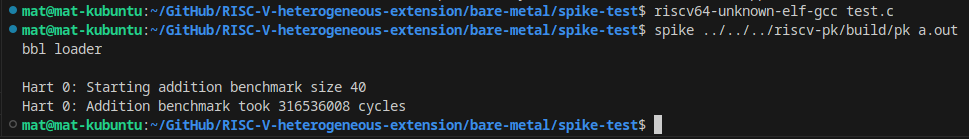
\includegraphics[width=\textwidth]{img/spike_output.png}
    \caption{Spike addition benchmark at size 40}
    \label{fig:spike_test_output}
\end{figure}

\section{Linux}
Adding Linux compatibility to the SoC would massively increase the potential use cases, and ease of use. While it is possible to compile programs to bare-metal code, this is very difficult and presents problems when users want to run high-level languages, such as Python, or run multiple programs at once. An OS running on the SoC would provide a huge number of features to the programmer and allow automatic SMP.

Some progress was made towards running Linux on the heterogeneous SoC. We identified the requirements for running a mainstream distribution of Linux and designed the CPUs to meet this minimum requirement. The requirements are lower for just the Linux kernel - if necessary, virtual memory can be disabled when compiling the kernel and this allows MMU-less CPUs to run the kernel, reducing the entry barrier. We created a Linux kernel config that didn't require an FPU, instead using softfloat to complete floating point calculations in software and compiled this for use on the B1S1 SoC. A supervisor binary interface is required for Linux to run, and we attempted to use OpenSBI, which was included in the vivado-risc-v\cite{vivado-risc-v} project. This was met with some success: OpenSBI was successfully started and the Linux kernel is started. The kernel identifies both CPUs in the system and begins setup, with SMP enabled. However, several illegal instruction errors occur while the file system is being initialised, and result in a failure to start the OS. 

An \texttt{initramfs} shell starts, which allows us some basic bash commands inside of a terminal, but this is a clear failure to run Linux.

\begin{figure}
    \centering
    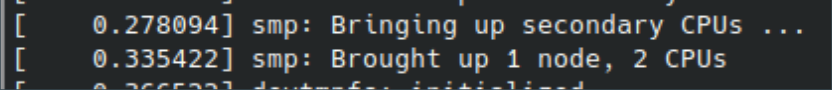
\includegraphics[width=\textwidth]{img/linux_smp.png}
    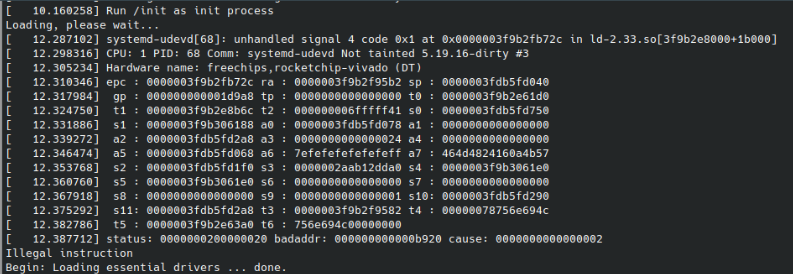
\includegraphics[width=\textwidth]{img/illegal_inst.png}
    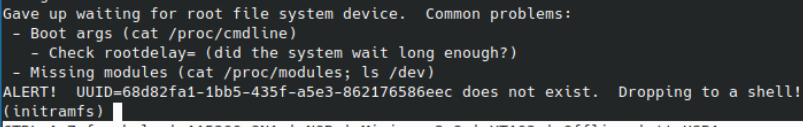
\includegraphics[width=\textwidth]{img/initramfs_shell.png}
    \caption{Attempts to run Linux}
    \label{fig:linux_attempt}
\end{figure}